% ICCSIS 2026 (Hangzhou, Nov 13-15, 2026) — ACM acmart template per conference Template.zip.
% Submission: https://paper-sub.com/paper/EEZ7VI  (deadline Aug 29, 2026; word+pdf)
% Checklist: >=8 pages single-column equivalent, CCS CONCEPTS, >=3 keywords,
% "Corresponding author" footnote, ORCID for all authors at publishing stage.
\documentclass[sigconf]{acmart}

\usepackage{booktabs}
\usepackage{listings}
\usepackage{tikz}
\usetikzlibrary{arrows.meta, positioning, fit, backgrounds}

\lstset{
  basicstyle=\ttfamily\footnotesize,
  breaklines=true,
  frame=single,
  columns=fullflexible
}

% Rights/conference placeholders — final values are set by the ICCSIS
% proceedings editor before camera-ready.
\setcopyright{none}
\acmConference[ICCSIS 2026]{2026 International Conference on Computer Science and Intelligent Systems}{November 13--15, 2026}{Hangzhou, China}
\acmBooktitle{2026 International Conference on Computer Science and Intelligent Systems (ICCSIS 2026)}
\acmPrice{}
\acmISBN{}
\acmDOI{}

\begin{document}

\title{Bridging the Enforcement Verification Gap: Detecting Divergence Between Declared and Actual Security Posture in Kubernetes Containerized Environments}

\author{Yehia Sobeh}
\authornote{Corresponding author.}
\affiliation{%
  \institution{Innopolis University}
  \city{Innopolis}
  \country{Russia}
}
\email{yehiasobehacm@gmail.com}

\author{Ruslan Damindarov}
\affiliation{%
  \institution{Innopolis University}
  \city{Innopolis}
  \country{Russia}
}
\affiliation{%
  \institution{Rubetek AI and Robotics Lab}
  \city{Innopolis}
  \country{Russia}
}
\email{r.damindarov@innopolis.university}
\email{r.damindarov@rubetek.com}

\author{Awwal Ishiaku}
\affiliation{%
  \institution{Innopolis University}
  \city{Innopolis}
  \country{Russia}
}
\email{a.ishiaku@innopolis.university}

\begin{abstract}
Container orchestration platforms such as Kubernetes rely on declarative security primitives to enforce security boundaries around containerized workloads. A fundamental assumption underlies this model: that the container runtime faithfully translates declared security intent into kernel-level enforcement. This paper identifies and addresses the \emph{enforcement verification gap}: the absence of tooling that systematically verifies whether declared Kubernetes security contexts are actually enforced by the container runtime. We present k8s-psa, a DaemonSet-based auditor that continuously compares pod security specifications retrieved from the Kubernetes API against the actual runtime state obtained through the container runtime interface. Through controlled experiments on a Minikube cluster with the Docker runtime, we evaluated the tool across seven test scenarios spanning fully hardened, partially secured, privileged, and deliberately misconfigured workloads. Our results reveal two categories of findings. First, privileged containers that declare seccomp system call filtering have that filtering silently stripped by the Docker runtime, a genuine enforcement gap that is invisible to existing specification-only tools. Second, the Docker runtime metadata interface omits the seccomp enforcement status of non-privileged containers that are correctly protected, an observability gap that produces false positives in naive runtime inspection. A kernel-verified cross-runtime validation on containerd shows that the enforcement gap generalizes, since containerd likewise strips declared seccomp profiles from privileged containers, whereas the observability gap is Docker-specific. These findings demonstrate that the enforcement verification gap is real, that it manifests differently across container configurations and runtimes, and that runtime inspection must account for the semantic differences between runtime metadata and actual kernel enforcement.
\end{abstract}

\begin{CCSXML}
<ccs2012>
 <concept>
  <concept_id>10002978.10003006.10003007.10003008</concept_id>
  <concept_desc>Security and privacy~Virtualization and security</concept_desc>
  <concept_significance>500</concept_significance>
 </concept>
 <concept>
  <concept_id>10002978.10002991.10002995</concept_id>
  <concept_desc>Security and privacy~Access control</concept_desc>
  <concept_significance>300</concept_significance>
 </concept>
</ccs2012>
\end{CCSXML}
\ccsdesc[500]{Security and privacy~Virtualization and security}
\ccsdesc[300]{Security and privacy~Access control}

\keywords{Kubernetes, container security, seccomp, runtime verification, enforcement drift, DevSecOps, security context}

\maketitle

\section{Introduction}

Modern software systems increasingly adopt microservice architectures deployed as containerized workloads on Kubernetes. This shift introduces security challenges that traditional perimeter-based approaches cannot address: a larger attack surface distributed across potentially hundreds of containers, complex dependency chains that pull in third-party images, and dynamic runtime behavior in which containers are continuously created, scaled, and terminated~\cite{wong2023, devipriya2023}.

Kubernetes addresses these challenges through declarative security primitives specified in pod security contexts. Admission controllers such as OPA Gatekeeper~\cite{gatekeeper2024} and Kyverno~\cite{kyverno2024} intercept pod creation requests and reject non-compliant specifications, while Pod Security Admission (PSA), which has been stable since Kubernetes v1.25~\cite{k8spsa2022}, enforces predefined security profiles at the namespace level.

Despite their differences, these tools share a critical limitation: every one of them reads security properties from the Kubernetes API, that is, from the \emph{declared} pod specification. None of them verifies that the container runtime has correctly translated those declarations into kernel-level enforcement. This verification matters because the translation from a Kubernetes pod specification to actual process isolation passes through multiple layers: the kubelet translates the pod specification into a Container Runtime Interface (CRI) request, the container runtime generates an Open Container Initiative (OCI) runtime specification, and a low-level runtime configures Linux kernel primitives~\cite{k8sseccomp2024}. Each translation step may add defaults, override values, or fail to apply certain restrictions.

This paper terms the resulting blind spot the \emph{enforcement verification gap} and presents k8s-psa,\footnote{Kubernetes Pod Security Auditor; not to be confused with the built-in Pod Security Admission (PSA) controller, which operates only on declared specifications.} a tool designed to detect divergences between declared security intent and actual runtime enforcement.

\subsection{Research Questions}

\begin{itemize}
    \item \textbf{RQ1:} To what extent does the actual security configuration of running containers diverge from the security properties declared in their Kubernetes pod specifications?
    \item \textbf{RQ2:} Can a lightweight, DaemonSet-based tool effectively detect such divergences with acceptable accuracy and performance overhead?
    \item \textbf{RQ3:} What categories of divergence occur in practice, and how should each category be classified from a security perspective?
\end{itemize}

\subsection{Contributions}

This work makes four contributions: (1)~a novel verification tool that closes the enforcement verification gap by systematically comparing declared Kubernetes security contexts against observed container runtime state; (2)~experimental evidence of enforcement drift in privileged containers, where both Docker and containerd strip declared seccomp profiles without warning, confirmed at the kernel level via \texttt{/proc/<pid>/status}; (3)~the discovery of an observability gap in the Docker runtime metadata interface, which causes correctly protected containers to appear unprotected and which does not occur on containerd; and (4)~an open-source evaluation framework comprising 44 unit tests, 7 deployment-level test cases, and a real-time dashboard.

\section{Background}

\subsection{Kubernetes Security Architecture}

Kubernetes enforces workload security through a layered model. The Kubernetes API accepts pod specifications containing \texttt{securityContext} fields that define the intended security posture~\cite{k8sseccomp2024}. The kubelet translates these specifications into CRI requests, from which the container runtime generates an OCI runtime specification~\cite{ocispec2023}, a JSON document describing the exact Linux kernel configuration. A low-level runtime then configures namespaces, cgroups, capabilities, and seccomp filters.

\subsection{Pod Security Admission and Policy Engines}

Pod Security Admission, which has been stable since Kubernetes v1.25~\cite{k8spsa2022}, enforces Pod Security Standards at admission time but does not monitor running workloads or verify runtime enforcement. Policy engines extend this admission-time model with periodic re-evaluation: OPA Gatekeeper~\cite{gatekeeper2024} audits cluster resources every 60 seconds, and Kyverno~\cite{kyverno2024} performs background scans every hour. In both cases, however, the audit reads the declared pod specification from the Kubernetes API, and neither tool queries the container runtime.

\subsection{Runtime Behavioral Monitoring}

At the opposite end of the stack, behavioral monitors such as Falco~\cite{falco2024} instrument the kernel via eBPF to detect anomalous system calls. These tools observe what containers \emph{do} at the kernel level, but they do not verify whether the active security configuration matches what was declared.

\section{Related Work}

\subsection{Static Misconfiguration Detection}

Research on Kubernetes security configuration has concentrated on the specification level. Rahman et al.~\cite{rahman2023} conducted a large-scale empirical study of 2,039 open-source Kubernetes manifests and explicitly identified runtime verification as future work. Building on the same specification-level view, Malul et al.~\cite{malul2024} proposed GenKubeSec, a fine-tuned language-model approach to YAML misconfiguration detection, and Sgan Cohen et al.~\cite{sgancohen2025} presented KubeGuard, which analyzes configuration files and runtime logs with a focus on RBAC and NetworkPolicy hardening; both works, which have not yet undergone peer review, likewise operate on declared configuration rather than enforced state.

\subsection{Configuration Drift Detection}

A second line of work targets configuration drift. Kubediff~\cite{kubediff2020} reports differences between the running Kubernetes state and version-controlled manifests. The Kubernetes blog~\cite{k8sdrift2021} described admission controllers for detecting container drift at runtime, and Komodor~\cite{komodor2023} documented operational approaches to drift detection. All of these approaches, however, treat the Kubernetes API as the source of truth for the running state; none extends below the API to the container runtime layer.

\subsection{The Identified Gap}

Several results indicate that the layer below the API deserves scrutiny. Kermabon-Bobinnec et al.~\cite{prospec2022} demonstrated that temporal inconsistency between the orchestration and runtime layers can be exploited to bypass security policies, and Shamim et al.~\cite{shamim2025} concluded that security researchers should investigate dynamic configuration violation detection. Survey work by Wong et al.~\cite{wong2023} and Devi Priya et al.~\cite{devipriya2023} likewise identified runtime configuration drift detection as under-explored. To the best of our knowledge, however, no existing open-source tool systematically compares the security declarations held by the Kubernetes API against the state reported by the container runtime. The present work addresses precisely this gap.

\section{Methodology}

\subsection{System Architecture}

k8s-psa operates as a Kubernetes DaemonSet~\cite{k8sdaemonset2024}, deploying one scanner pod per cluster node. This deployment model guarantees complete node coverage, co-locates each scanner with the local container runtime socket, and scales automatically as nodes join or leave the cluster. Each instance performs periodic two-layer security scans; Fig.~\ref{fig:pipeline} shows the scanning pipeline.

\textbf{Layer~1 (Spec Check)} reads pod specifications from the Kubernetes API and checks them against eight configurable security policies (privileged mode, root user, host PID/network/IPC, seccomp profile, dangerous capabilities, and read-only root filesystem). This layer is functionally equivalent to existing policy engines and serves two purposes: it provides a baseline against which Layer~2 findings can be contextualized, and it flags pods that lack security declarations entirely, a case Layer~2 cannot detect, because the absence of a declaration leaves no intent to verify.

\textbf{Layer~2 (Drift Detection)}, the novel contribution, compares declared specifications against actual runtime state by: (1)~extracting a \texttt{SpecSecurityState} from the Kubernetes API; (2)~querying the container runtime (\texttt{docker inspect} or \texttt{crictl inspect}) to build a \texttt{RuntimeSecurityState}; (3)~normalizing both states to account for expected divergences; and (4)~comparing the normalized states field by field across seven security dimensions.

The comparison engine classifies each divergence as \textbf{CRITICAL} (a declared restriction is absent at runtime), \textbf{WARNING} (an undeclared capability is present), or \textbf{INFO} (the runtime is more restrictive than declared).

\textbf{Reporting pipeline.} Both layers emit their findings into a common reporting stage. An AlertManager consolidates the \texttt{spec\_violations} produced by Layer~1 and the \texttt{drift\_findings} produced by Layer~2, appends each record as one line of newline-delimited JSON to \texttt{findings.jsonl}, and exposes a lightweight dashboard over HTTP (port~8080) that renders the current findings for operators. This reporting stage forms the lower portion of Fig.~\ref{fig:pipeline}.

\begin{figure}[htbp]
\centering
\resizebox{\columnwidth}{!}{%
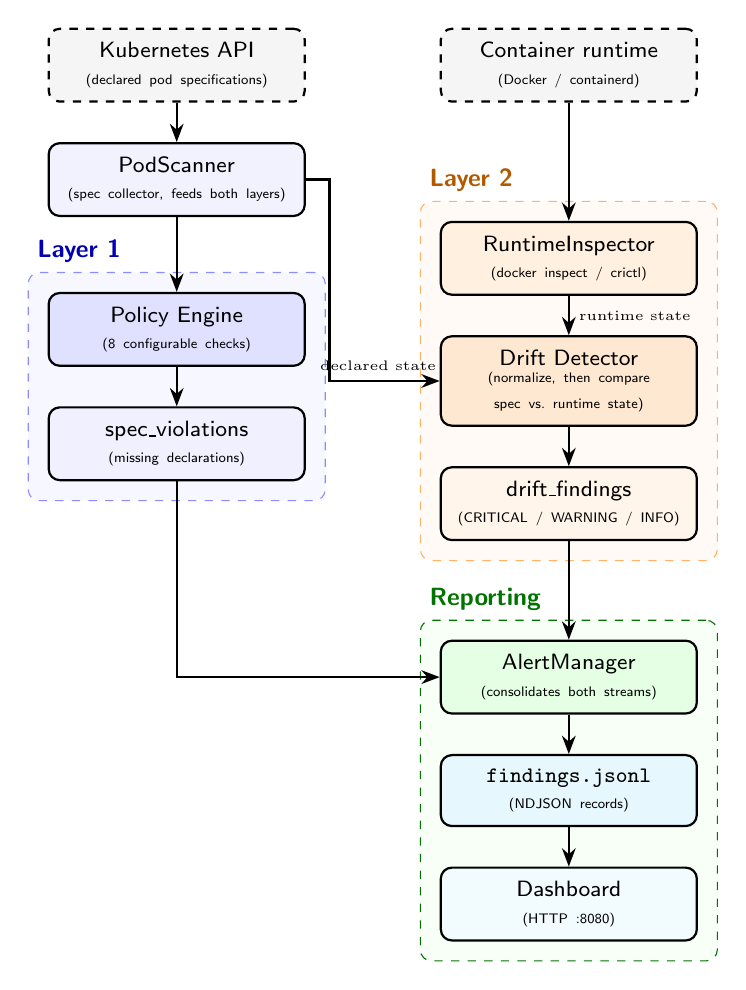
\begin{tikzpicture}[
    node distance = 0.5cm and 0.9cm,
    block/.style = {
      draw, thick, rounded corners,
      text width=2.9cm, align=center,
      inner sep=5pt,
      font=\sffamily\footnotesize
    },
    arrow/.style = {->, >=Stealth, thick},
    grp/.style = {draw, dashed, rounded corners, inner sep=7pt},
]
% data sources
\node[block, dashed, fill=gray!8] (api) {Kubernetes API\\\tiny(declared pod specifications)};
\node[block, dashed, fill=gray!8, right=1.7cm of api] (rt) {Container runtime\\\tiny(Docker / containerd)};

% shared spec collector
\node[block, fill=blue!5, below=of api] (pod) {PodScanner\\\tiny(spec collector, feeds both layers)};

% Layer 1 path
\node[block, fill=blue!12, below=0.95cm of pod] (pol) {Policy Engine\\\tiny(8 configurable checks)};
\node[block, fill=blue!6, below=of pol] (spec) {spec\_violations\\\tiny(missing declarations)};

% Layer 2 path (RuntimeInspector aligned with the Policy Engine row)
\node[block, fill=orange!12, below=1.5cm of rt] (insp) {RuntimeInspector\\\tiny(docker inspect / crictl)};
\node[block, fill=orange!18, below=of insp] (drift) {Drift Detector\\\tiny(normalize, then compare\\\tiny spec vs.\ runtime state)};
\node[block, fill=orange!8, below=of drift] (find) {drift\_findings\\\tiny(CRITICAL / WARNING / INFO)};

% reporting pipeline
\node[block, fill=green!10, below=1.25cm of find.south] (alert) {AlertManager\\\tiny(consolidates both streams)};
\node[block, fill=cyan!10, below=of alert] (ndjson) {\texttt{findings.jsonl}\\\tiny(NDJSON records)};
\node[block, fill=cyan!5, below=of ndjson] (dash) {Dashboard\\\tiny(HTTP :8080)};

% arrows
\draw[arrow] (api) -- (pod);
\draw[arrow] (rt) -- (insp);
\draw[arrow] (pod) -- (pol);
\draw[arrow] (pol) -- (spec);
\draw[arrow] (insp) -- node[right, font=\tiny] {runtime state} (drift);
\draw[arrow] (pod.east) -- ++(0.30,0) |- node[pos=0.72, above, font=\tiny] {declared state} (drift.west);
\draw[arrow] (drift) -- (find);
\draw[arrow] (spec.south) |- (alert.west);
\draw[arrow] (find.south) -- (alert.north);
\draw[arrow] (alert) -- (ndjson);
\draw[arrow] (ndjson) -- (dash);

% grouping of the two scan layers and the reporting stage
\begin{scope}[on background layer]
  \node[grp, draw=blue!45,        fill=blue!3,   fit=(pol)(spec)]          (l1box) {};
  \node[grp, draw=orange!60,      fill=orange!4, fit=(insp)(drift)(find)]  (l2box) {};
  \node[grp, draw=green!45!black, fill=green!3,  fit=(alert)(ndjson)(dash)](rpbox) {};
\end{scope}
\node[font=\sffamily\bfseries\small, blue!70!black,   anchor=south west] at (l1box.north west) {Layer 1};
\node[font=\sffamily\bfseries\small, orange!70!black, anchor=south west] at (l2box.north west) {Layer 2};
\node[font=\sffamily\bfseries\small, green!45!black,  anchor=south west] at (rpbox.north west) {Reporting};
\end{tikzpicture}%
}
\caption{Two-layer scanning pipeline of k8s-psa. The PodScanner is a shared spec collector: it reads declared specifications from the Kubernetes API and feeds both layers. Layer~1 validates those specifications against eight policies and reports missing declarations. Layer~2, the novel contribution, additionally obtains the actual runtime state through the RuntimeInspector, normalizes both states, and compares them field by field to detect divergence between declared and enforced security. The AlertManager then consolidates the two finding streams, appends them as NDJSON records to \texttt{findings.jsonl}, and the dashboard serves those records over HTTP for inspection.}
\label{fig:pipeline}
\end{figure}

\subsection{Capability Normalization}

Naive comparison of declared and observed capability sets would flood the operator with false positives, because the container runtime adds 14 default Linux capabilities to every non-privileged container~\cite{dockerseccomp2024}. The normalizer therefore computes the \emph{expected} capability set from the pod specification: it starts with these documented defaults, removes the capabilities listed in \texttt{drop}, and adds those listed in \texttt{add}. Only deviations from this expected set generate findings.

\subsection{Experimental Environment}
\label{sec:env}

Experiments were conducted on a single-node Minikube cluster (v1.35.0) running Kubernetes v1.32.0 with Docker 27.4.1. The host machine was a laptop with an Intel Core i5-1135G7 processor (4 cores, 8 threads, up to 4.2\,GHz) and 8\,GB of RAM, running Ubuntu 22.04.5 LTS with Linux kernel 6.8; the Minikube node was allocated 2 vCPUs and 2200\,MB of memory through the Docker driver. The scanner interval was 60 seconds. Seven test pods were designed to cover the spectrum of security configurations: fully hardened, no security context, privileged with and without a declared seccomp profile, partially secured, one with privilege escalation restricted, and one sharing host namespaces. Three scan cycles were captured per pod. In addition to the seven purpose-built pods, the scanner observed the Kubernetes control plane pods running in the cluster, which serve as unplanned real-world subjects. Table~\ref{tab:specs} summarizes the hardware and software configuration.

\begin{table}[htbp]
\caption{Experimental System Specifications}
\label{tab:specs}
\centering
\begin{tabular}{ll}
\toprule
\textbf{Component} & \textbf{Specification} \\
\midrule
Host CPU        & Intel Core i5-1135G7 (4C/8T, up to 4.2\,GHz) \\
Host memory     & 8\,GB \\
Host OS         & Ubuntu 22.04.5 LTS \\
Host kernel     & Linux 6.8 \\
Minikube        & v1.35.0 (Docker driver) \\
Node resources  & 2 vCPUs, 2200\,MB memory \\
Kubernetes      & v1.32.0 \\
Primary runtime & Docker 27.4.1 \\
Cross-runtime   & containerd 1.7.24, runc 1.2.2 \\
Scan interval   & 60\,s \\
\bottomrule
\end{tabular}
\end{table}

To test whether the findings are Docker-specific, we additionally performed a targeted cross-runtime validation on a second cluster on the same host, with the identical Kubernetes version (v1.32.0) and resource allocation but the containerd runtime (containerd 1.7.24, runc 1.2.2), redeploying the decisive test pods (1, 3, and~4) and verifying enforcement both through \texttt{crictl inspect} and directly against the kernel via \texttt{/proc/<pid>/status}.

\section{Results}

\subsection{Detection Results Summary}

Table~\ref{tab:results} presents the Layer~2 drift findings for each test pod. Layer~1 behaved as expected across all seven pods (e.g., zero violations for the fully hardened Pod~1 and six violations for the host-namespace Pod~7) and is not discussed further; the remainder of this section focuses on the Layer~2 findings that constitute the contribution of this work.

\begin{table}[htbp]
\caption{Layer~2 Drift Findings by Test Pod}
\label{tab:results}
\centering
\begin{tabular}{lcccc}
\toprule
\textbf{Test Pod} & \textbf{CRIT} & \textbf{WARN} & \textbf{INFO} & \textbf{Match} \\
\midrule
1. Fully Hardened   & 1*  & 0  & 0 & \S\ref{sec:obsgap} \\
2. No Security Ctx  & 0   & 0  & 0 & Yes \\
3. Priv + Seccomp   & 1   & 27 & 0 & Yes \\
4. Priv, No Seccomp & 0   & 27 & 0 & Yes \\
5. Partial Security & 1*  & 0  & 0 & \S\ref{sec:obsgap} \\
6. No Privesc       & 1*  & 0  & 0 & \S\ref{sec:obsgap} \\
7. Host Namespaces  & 0   & 0  & 2 & Yes \\
\bottomrule
\multicolumn{5}{l}{\footnotesize *Observability false positives analyzed in Section~\ref{sec:obsgap}.}
\end{tabular}
\end{table}

\subsection{True Positive: Privileged Seccomp Stripping}

The central finding concerns Test Pod~3, which declares both \texttt{privileged: true} and \texttt{seccompProfile.type: RuntimeDefault}. For such containers, the Docker runtime grants all 41 Linux capabilities and removes the seccomp filter entirely, even though seccomp filtering is explicitly declared. This behavior is documented in the Moby project issue tracker~\cite{moby41321}. The tool reported the divergence as follows:

\begin{lstlisting}
{
  "field": "seccompProfile",
  "severity": "critical",
  "category": "seccomp_mismatch",
  "description": "Spec declares seccomp type
    'RuntimeDefault' but the runtime has NO
    seccomp filter (unconfined)",
  "declared": "RuntimeDefault",
  "actual": "unconfined (null)"
}
\end{lstlisting}

Test Pod~4 serves as the experimental control: it has the same runtime state as Pod~3 but no seccomp declaration, and it produced zero CRITICAL findings. The 27 WARNING-level capability findings are identical between Pods~3 and~4, reflecting the 27 capabilities that privileged mode grants beyond the 14 defaults, including \texttt{CAP\_SYS\_ADMIN}, \texttt{CAP\_NET\_ADMIN}, and \texttt{CAP\_SYS\_MODULE}.

The security implication is direct. An operator who declares \texttt{RuntimeDefault} on a privileged container reasonably expects system call filtering to be active. Any specification-only tool reads the Kubernetes API, sees \texttt{RuntimeDefault}, and reports the container as filtered. Only by querying the container runtime does this removal become visible.

\subsection{Observability Gap}
\label{sec:obsgap}

Test Pods~1, 5, and~6, all non-privileged and all declaring \texttt{RuntimeDefault}, unexpectedly produced CRITICAL seccomp findings. Investigation revealed that these are false positives caused by a documented but widely misunderstood behavior of the Docker metadata interface. When cri-dockerd translates \texttt{RuntimeDefault}, it passes no explicit \texttt{SecurityOpt} entry to Docker and instead relies on Docker's implicit default profile~\cite{dockerseccomp2024}, which restricts several dozen sensitive system calls such as \texttt{mount}, \texttt{ptrace}, and \texttt{reboot}~\cite{datadog2023}. Because the implicit profile never appears in \texttt{docker inspect} output, a correctly protected container is indistinguishable at the metadata level from an unprotected one. The CIS Docker Benchmark (check 5.21) documents exactly this semantics: an empty \texttt{SecurityOpt} field indicates that the default profile is \emph{active}, not that seccomp is disabled~\cite{cisdocker2024, moric2025}.

The Kubernetes control plane pods observed during the evaluation (etcd, kube-apiserver, kube-controller-manager, kube-scheduler) exhibited the same phenomenon, each producing one false-positive CRITICAL seccomp finding. This consistency across purpose-built and real-world workloads confirms that the observability gap is systematic rather than an artifact of the test pod design.

\subsection{Pod~3 vs.\ Pod~4: Controlled Comparison}

Table~\ref{tab:comparison} presents the controlled comparison between Pod~3 and Pod~4, which isolates the seccomp declaration as the single independent variable.

\begin{table}[htbp]
\caption{Controlled Comparison: Pod~3 vs.\ Pod~4}
\label{tab:comparison}
\centering
\begin{tabular}{lcc}
\toprule
\textbf{Property} & \textbf{Pod 3} & \textbf{Pod 4} \\
\midrule
Spec: privileged     & true & true \\
Spec: seccompProfile & RuntimeDefault & Not declared \\
Runtime: capabilities & All 41 & All 41 \\
Runtime: seccomp     & Unconfined & Unconfined \\
L2 CRITICAL          & \textbf{1} & \textbf{0} \\
L2 WARNING           & 27 & 27 \\
\bottomrule
\end{tabular}
\end{table}

Both pods have identical runtime states; the only difference is the seccomp declaration. The drift detector flags Pod~3 and remains silent on Pod~4, demonstrating its \emph{specificity}: the tool distinguishes ``restriction declared but not enforced'' from ``restriction never declared.''

\subsection{Cross-Runtime Validation on containerd}
\label{sec:crossruntime}

Table~\ref{tab:crossruntime} summarizes the validation experiment on the containerd cluster, with the kernel's own seccomp status as ground truth.

\begin{table}[htbp]
\caption{Cross-Runtime Validation (containerd 1.7.24, runc 1.2.2)}
\label{tab:crossruntime}
\centering
\begin{tabular}{lccc}
\toprule
\textbf{Check} & \textbf{Pod 1} & \textbf{Pod 3} & \textbf{Pod 4} \\
\midrule
OCI spec: seccomp     & Present & Absent & Absent \\
OCI spec: capabilities & 0 & 41 & 41 \\
Kernel: \texttt{Seccomp} field & \textbf{2} (filter) & \textbf{0} (none) & \textbf{0} (none) \\
Kernel: \texttt{CapBnd} bits  & 0 & 41 & 41 \\
\bottomrule
\end{tabular}
\end{table}

Two conclusions follow. First, \emph{the enforcement gap generalizes beyond Docker}: Pod~3's declared \texttt{RuntimeDefault} profile is passed by the kubelet through the CRI but stripped by containerd, and the kernel confirms that no filter is installed (\texttt{Seccomp:~0}). The paper's central finding is therefore not a Docker quirk: it holds on the runtime that dominates production clusters. Second, \emph{the observability gap is Docker-specific}: \texttt{crictl inspect} on containerd exposes the full OCI runtime specification, in which Pod~1's seccomp allowlist is explicitly visible and matches the kernel state (\texttt{Seccomp:~2}). The false positives observed on Docker would not occur on containerd.

The validation also surfaced a further metadata-semantics trap: in the CRI protobuf JSON, a seccomp profile of type \texttt{RuntimeDefault} serializes as an empty object (enum value~0 is omitted), so naive inspection of the CRI configuration would misread a correctly declared profile as absent. This reinforces the paper's argument that verification tools must interpret runtime metadata semantics rather than take them at face value.

\subsection{Performance Characteristics}

On the experimental system detailed in Section~\ref{sec:env} and Table~\ref{tab:specs} (Intel Core i5-1135G7, 8\,GB RAM, Minikube node limited to 2 vCPUs and 2200\,MB), each scan cycle completed in approximately 3.1 seconds for 16 pods (0.7~s for Layer~1 and 2.4~s for Layer~2 across 18 containers), well within the 60-second scan interval. The scanner consumed 64~MiB of memory and fewer than 100m CPU, and the dashboard a further 32~MiB. The tool ships with 44 automated unit tests that execute in 0.2 seconds.

\section{Discussion}

\subsection{Answers to the Research Questions}

\textbf{RQ1 (extent of divergence).} Divergence between declared and enforced security is not hypothetical. Privileged containers with seccomp declarations exhibit a real enforcement gap in which the runtime drops the declared restriction unannounced, on Docker and containerd alike, and privileged mode inflates the capability set by 27 capabilities beyond the declared expectation.

\textbf{RQ2 (feasibility of lightweight detection).} A DaemonSet-based tool can detect such divergences with modest resources (64~MiB, $<$100m CPU, 3.1~s per cycle). The controlled Pod~3/Pod~4 comparison shows that detection is specific rather than merely sensitive; the observability false positives show that accuracy depends on correctly interpreting runtime metadata semantics.

\textbf{RQ3 (categories of divergence).} Three categories emerged: (1)~a \emph{genuine enforcement gap} (CRITICAL), where a declared seccomp profile is stripped by privileged mode; (2)~\emph{capability inflation} (WARNING), where privileged mode grants all 41 capabilities; and (3)~an \emph{observability gap} (false-positive CRITICAL), where Docker's implicit seccomp default is invisible to metadata inspection.

\subsection{The Gap Is Real but Nuanced}

The results therefore confirm the enforcement verification gap while revealing that it has two distinct forms. The enforcement gap creates a false sense of security, because the declared control simply is not there, and the cross-runtime validation shows it is systemic rather than an implementation quirk of one runtime. The observability gap, by contrast, is a property of the Docker metadata interface, and it demonstrates that runtime metadata is a lossy abstraction over kernel state. A definitive verdict requires reading the kernel's own enforcement status from \texttt{/proc/<pid>/status}, where a \texttt{Seccomp} value of~2 confirms that BPF filter mode is active~\cite{kep2413}; our validation experiment used exactly this check as ground truth.

\subsection{Comparison with Existing Tools}

Table~\ref{tab:tools} positions k8s-psa in the existing tool landscape. To the best of our knowledge, no existing open-source tool performs the spec-versus-runtime comparison that k8s-psa implements: OPA Gatekeeper~\cite{gatekeeper2024} and Kyverno~\cite{kyverno2024} read only the Kubernetes API, Falco~\cite{falco2024} monitors kernel behavior without spec comparison, and Kubediff~\cite{kubediff2020} reports differences between the API state and git manifests. k8s-psa occupies the space between specification-level tools and kernel-level monitors.

\begin{table}[htbp]
\caption{Positioning of k8s-psa Among Existing Tools}
\label{tab:tools}
\centering
\begin{tabular}{lll}
\toprule
\textbf{Tool} & \textbf{What It Checks} & \textbf{Layer} \\
\midrule
OPA Gatekeeper & Spec vs.\ policy constraints & API only \\
Kyverno        & Spec vs.\ validate rules & API only \\
Falco          & Syscall behavior (eBPF) & Kernel only \\
Kubediff       & Spec vs.\ git manifests & API vs.\ git \\
\textbf{k8s-psa} & \textbf{Spec vs.\ runtime state} & \textbf{API vs.\ runtime} \\
\bottomrule
\end{tabular}
\end{table}

\subsection{Limitations}

Five limitations bound the generality of these results. First, the full tool evaluation ran on Docker; the containerd validation covered the three decisive pods rather than the complete scenario matrix, and CRI-O remains untested. Second, the tool's automated seccomp verification relies on runtime metadata rather than kernel-level status (the kernel check in Section~\ref{sec:crossruntime} was performed manually and is not yet integrated into the scanner). Third, the evaluation was conducted on single-node clusters. Fourth, the tool shells out to CLI commands rather than using native API client libraries. Fifth, seven test pods cover the primary security dimensions but not every configuration (e.g., init, sidecar, or ephemeral containers).

\subsection{Future Work}

Three directions merit investigation: integrating the \texttt{/proc/<pid>/status} kernel check, validated manually in this work, into the scanner itself, which would eliminate the observability gap entirely; extending the cross-runtime study to CRI-O and managed multi-node clusters (GKE, EKS) together with a prevalence study over real-world workloads; and investigating whether mutating admission webhooks introduce additional enforcement gaps by modifying security contexts after user submission.

\section{Conclusion}

This paper identified and addressed the enforcement verification gap in Kubernetes security. Through controlled experiments, we demonstrated that privileged containers declaring seccomp filtering had that filtering silently removed by the container runtime, on Docker and, as our kernel-verified cross-runtime validation shows, on containerd as well. This is a real enforcement failure that is invisible to all existing specification-only tools. We additionally discovered an observability gap in Docker's metadata interface that makes correctly protected containers appear unprotected; on containerd this gap does not occur. The tool, its evaluation framework, and its real-time dashboard are provided as open-source contributions.

\begin{acks}
The authors gratefully acknowledge the support of the Laboratory for Robotics and Artificial Intelligence and the Institute of Information Security at Innopolis University, together with the Rubetek AI and Robotics Lab.
\end{acks}

\bibliographystyle{ACM-Reference-Format}
\bibliography{refs}

\end{document}
